\section{Wavelet transforms}

\begin{frame} \frametitle{Wavelet transforms for EXAFS analysis}

\begin{cenpage}{105mm}

  The Fourier transform is fundamental to understanding EXAFS.

  Wavelet transforms extend Fourier transforms, mixing $k$ and $R$.

  They have been used by a handful of groups.



\end{cenpage}

\begin{columns}
  \begin{column}[T]{70mm}

    {\onslide+<2->  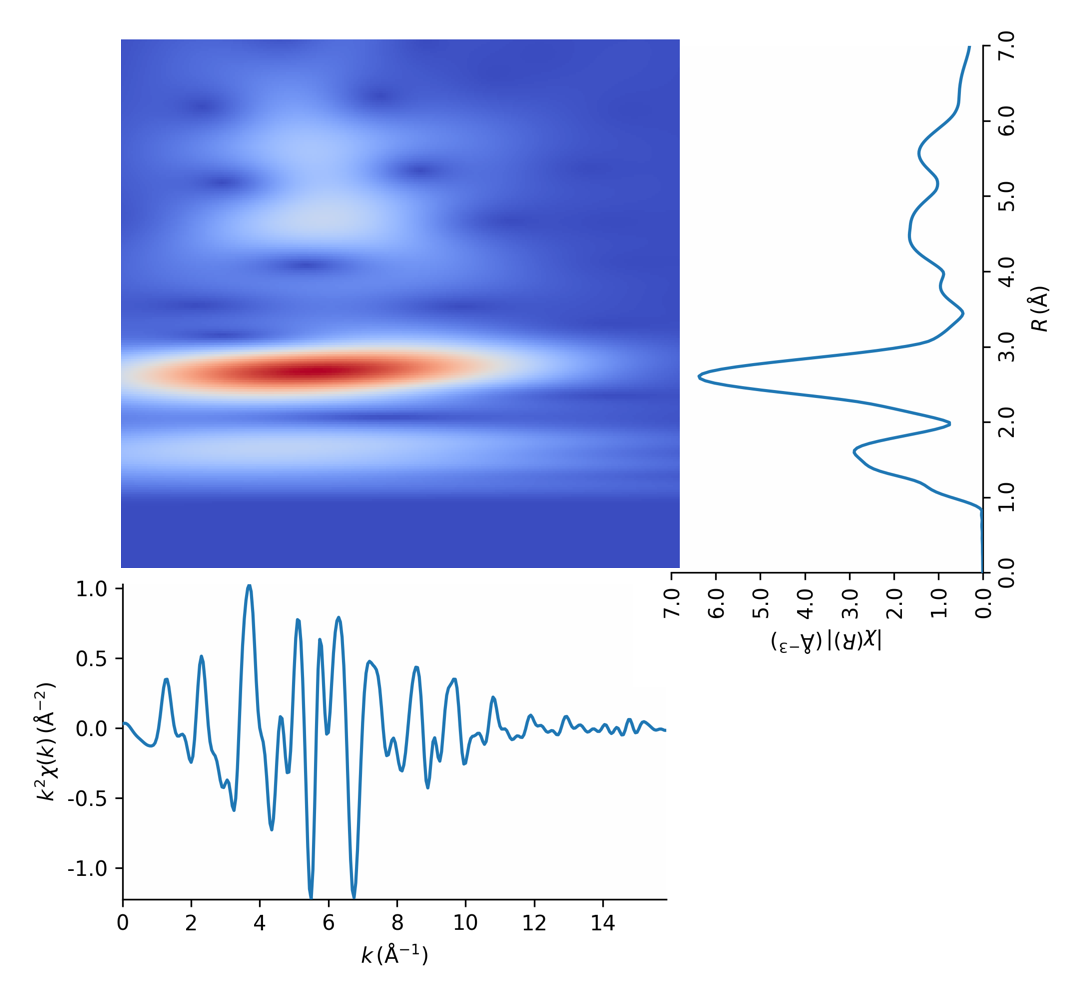
\includegraphics[width=70mm]{figs/wavelets/wavelet_composite_mag}  }

  \end{column}

\begin{column}[T]{52mm}

  {\onslide+<2-> 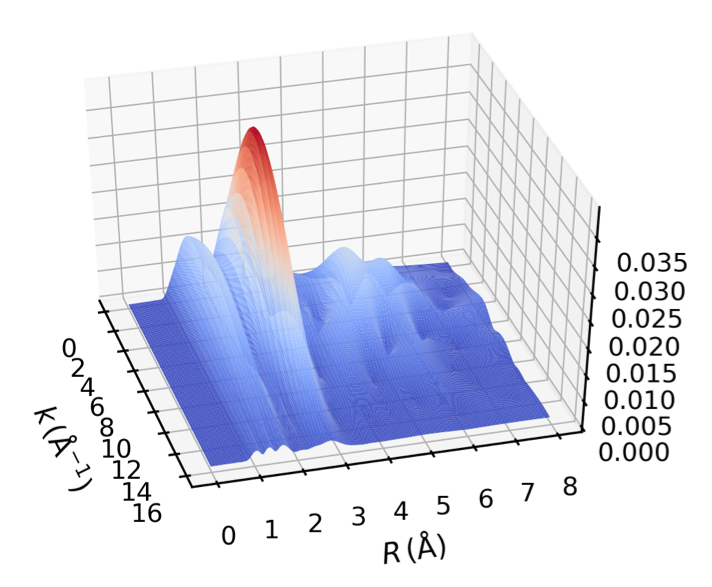
\includegraphics[width=52mm]{figs/wavelets/wavelet_surface} }

  \vmm

  Wavelet transform for FeO data.

  \vmm \vmm

{\hspace{-15mm}{
    {\onslide+<2->
    \begin{minipage}{60mm}
      {\tiny{
          This is using the ``Continuous Cauchy'' wavelet transform, as
          described by Munoz, Argoul, and Farges, {\emph{Am Mineralogist}},
          2003

          Others (Funke {\emph{et al}}, Penfold, {\emph{et al}}) have used Morlet
          wavelets.
        }}
  \end{minipage}
}
}}


  \end{column}

\end{columns}
\end{frame}
